\section{Experiment Setup}

%The aim of our experiment is to determine whether dynamic DOF has a significant effect on visual discomfort on the Oculus. 

% I am not sure on this section. It explains the algorithm used, but I am not confident that the explanation is any good.
We implement real-time dynamic DoF using the GPU as in~\cite{riguer04, duchowski14}. Given that around 86\% of a user's fixation time, and 82\% of total viewing time is spent looking the centre of the screen~\cite{kenney05}, we assume the user's gaze will always be concentrated in the centre of the screen and thus keep that point in focus. Our DoF implementation is based around the bokeh implementation provided in UE4 to support fast solutions with reasonable visual quality~\cite{ue4Bokeh}. \\

%REWORDING START
%For exach pixel on the screen, we cast a ray from the user's virtual camera to the scene to find the depth of the object at that pixel., We define $d_{max}$ as the longest possible focal distance in the scene, $d_{min}$ as the shortest, $d_{centre}$ as the depth at the centre of the screen, $p_{long}$ as the world space distance between the objects at $d_{max}$ and $d_{centre}$ and $p_{short}$ as the world space distance between the objects at $d_{min}$ and $d_{centre}$.\\
We implement bokeh DoF by using an approach based on \say{circles of confusion}~\cite{riguer04}. To begin, we find the depth $d_f$, of the object that is supposed to be in focus (at the centre of the screen). This is difficult to determine given the low resolution of the Oculus screen compared to its proximity to users eyes. We cannot be sure that the reported object depth is the correct focal depth with only one ray: if there is only a very small gap between two objects, as in Fig.~\ref{fig:raycast}, it is highly likely that the user is focusing on the foreground objects. To compensate for this, we cast random rays with small, random angular deviations into the scene, and then estimate $d_f$ using the set of reported depths. 

\begin{figure}[h!]
       \centering
           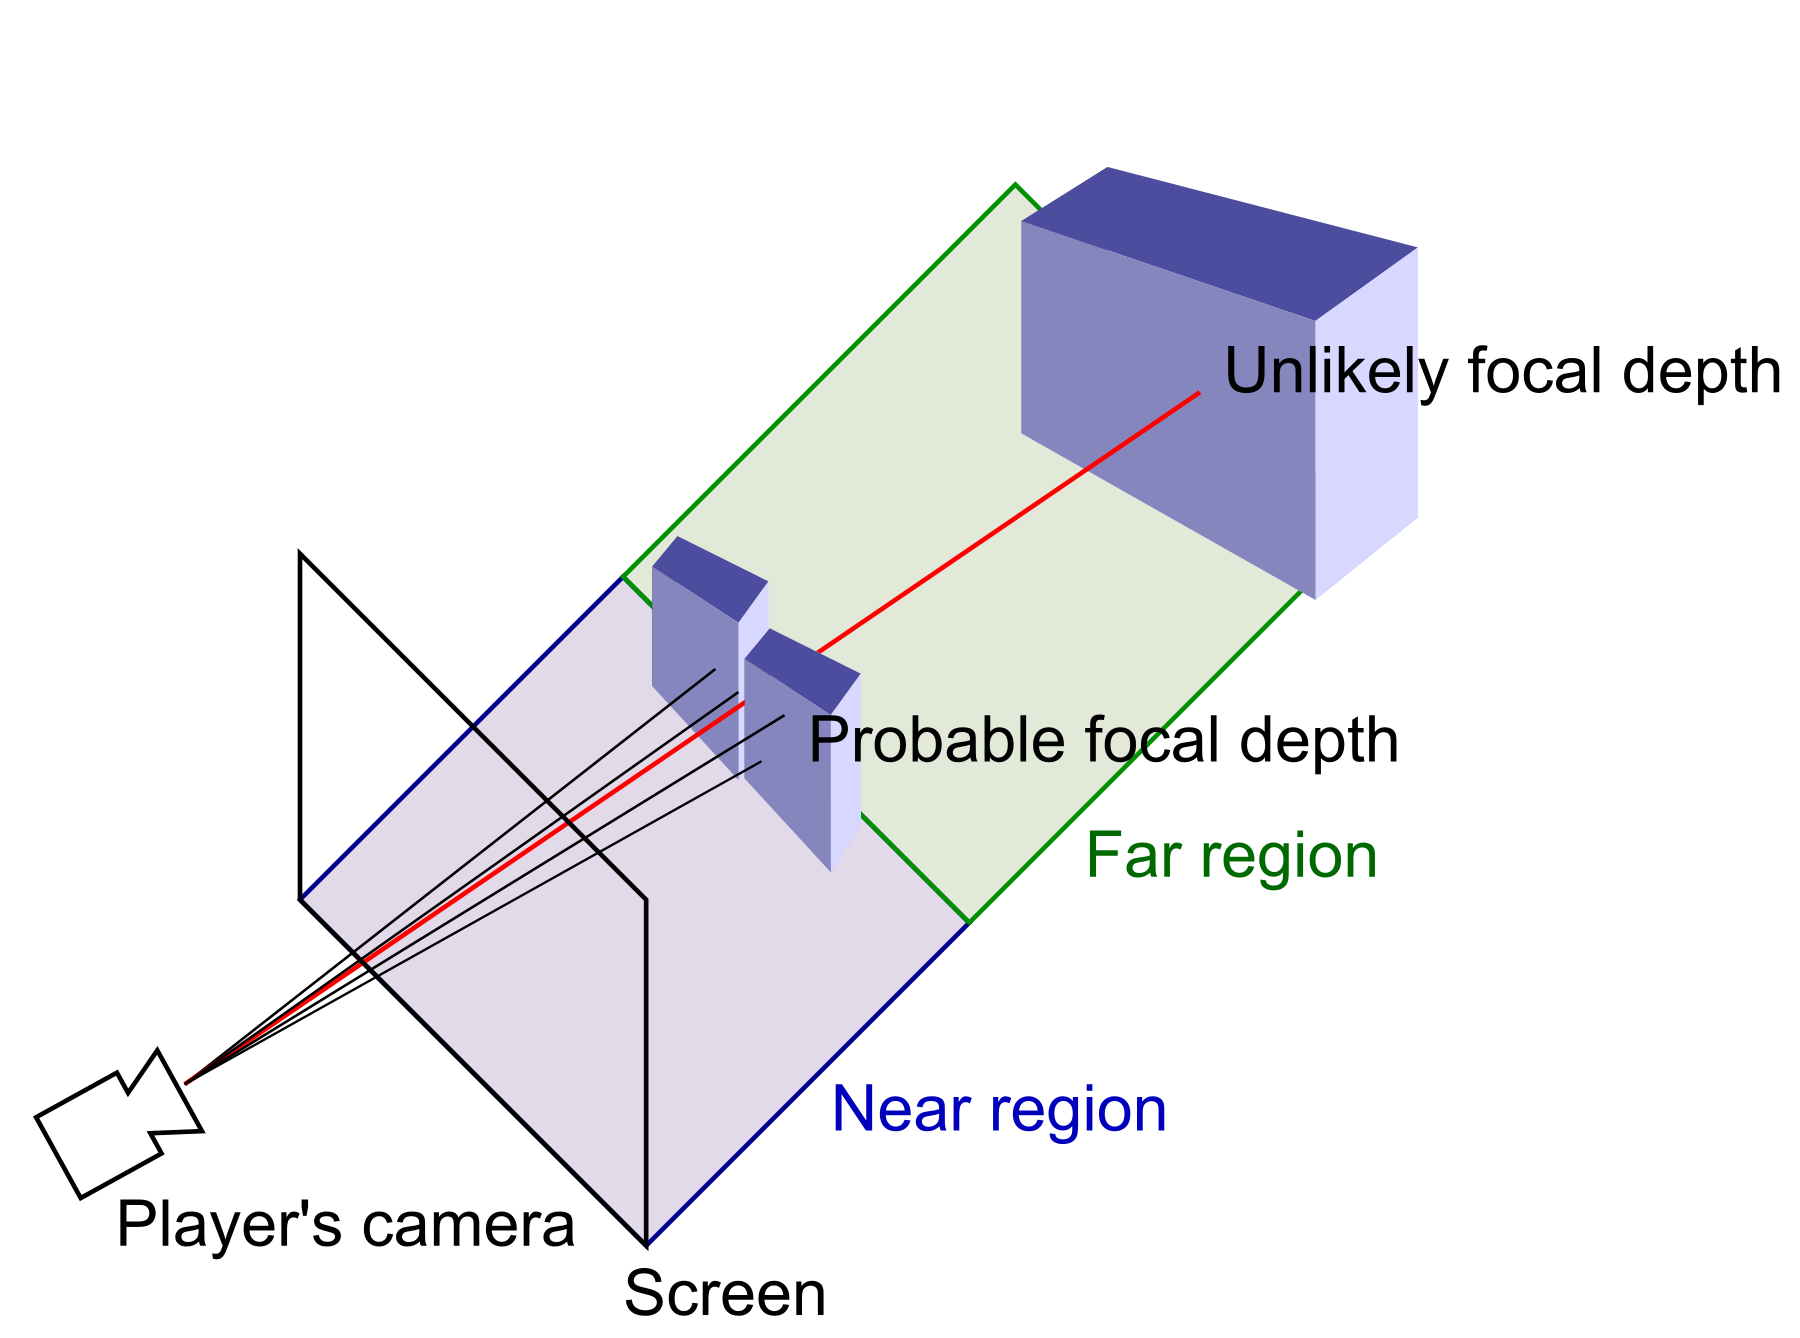
\includegraphics[width=0.45\textwidth]{images/distanceCheck.png}
            \caption{In order to avoid focusing at unlikely depths (red), multiple rays (black) are cast to find $d_f$ .}
            \label{fig:raycast}
\end{figure}

For each pixel, we find the depth $d_p$ of the object under that pixel. In order to avoid \say{bleeding effects} we split the screen into two regions: near and far, before convolving the set of pixels in each of these regions against a circular blur kernel with a fluctuating radius $r \propto | d_f - d_p |$. The opacity of the kernel is inversely proportional to $r$. These regions are then merged to create the completed frame. We do not immediately change $d_f$ when participants move or look around. Instead, we interpolate the change in focal distance based on the refocusing speed of the human eye~\cite{sun88} to more accurately mimic behaviours of the human visual system. We selected the radius $r$ using a preliminary experiment where a test environment was generated consisting of multiple identical objects at differing visual depths, as shown in Fig.~\ref{fig:testScene}. Through visual analysis of this scene, $r$ was selected to be 1.75\% of the screen width. We assume a fixed inter-pupillary distance (IPD) equal to the average value for adults.  \\
%
%\begin{figure}[h!]
%        \centering
%            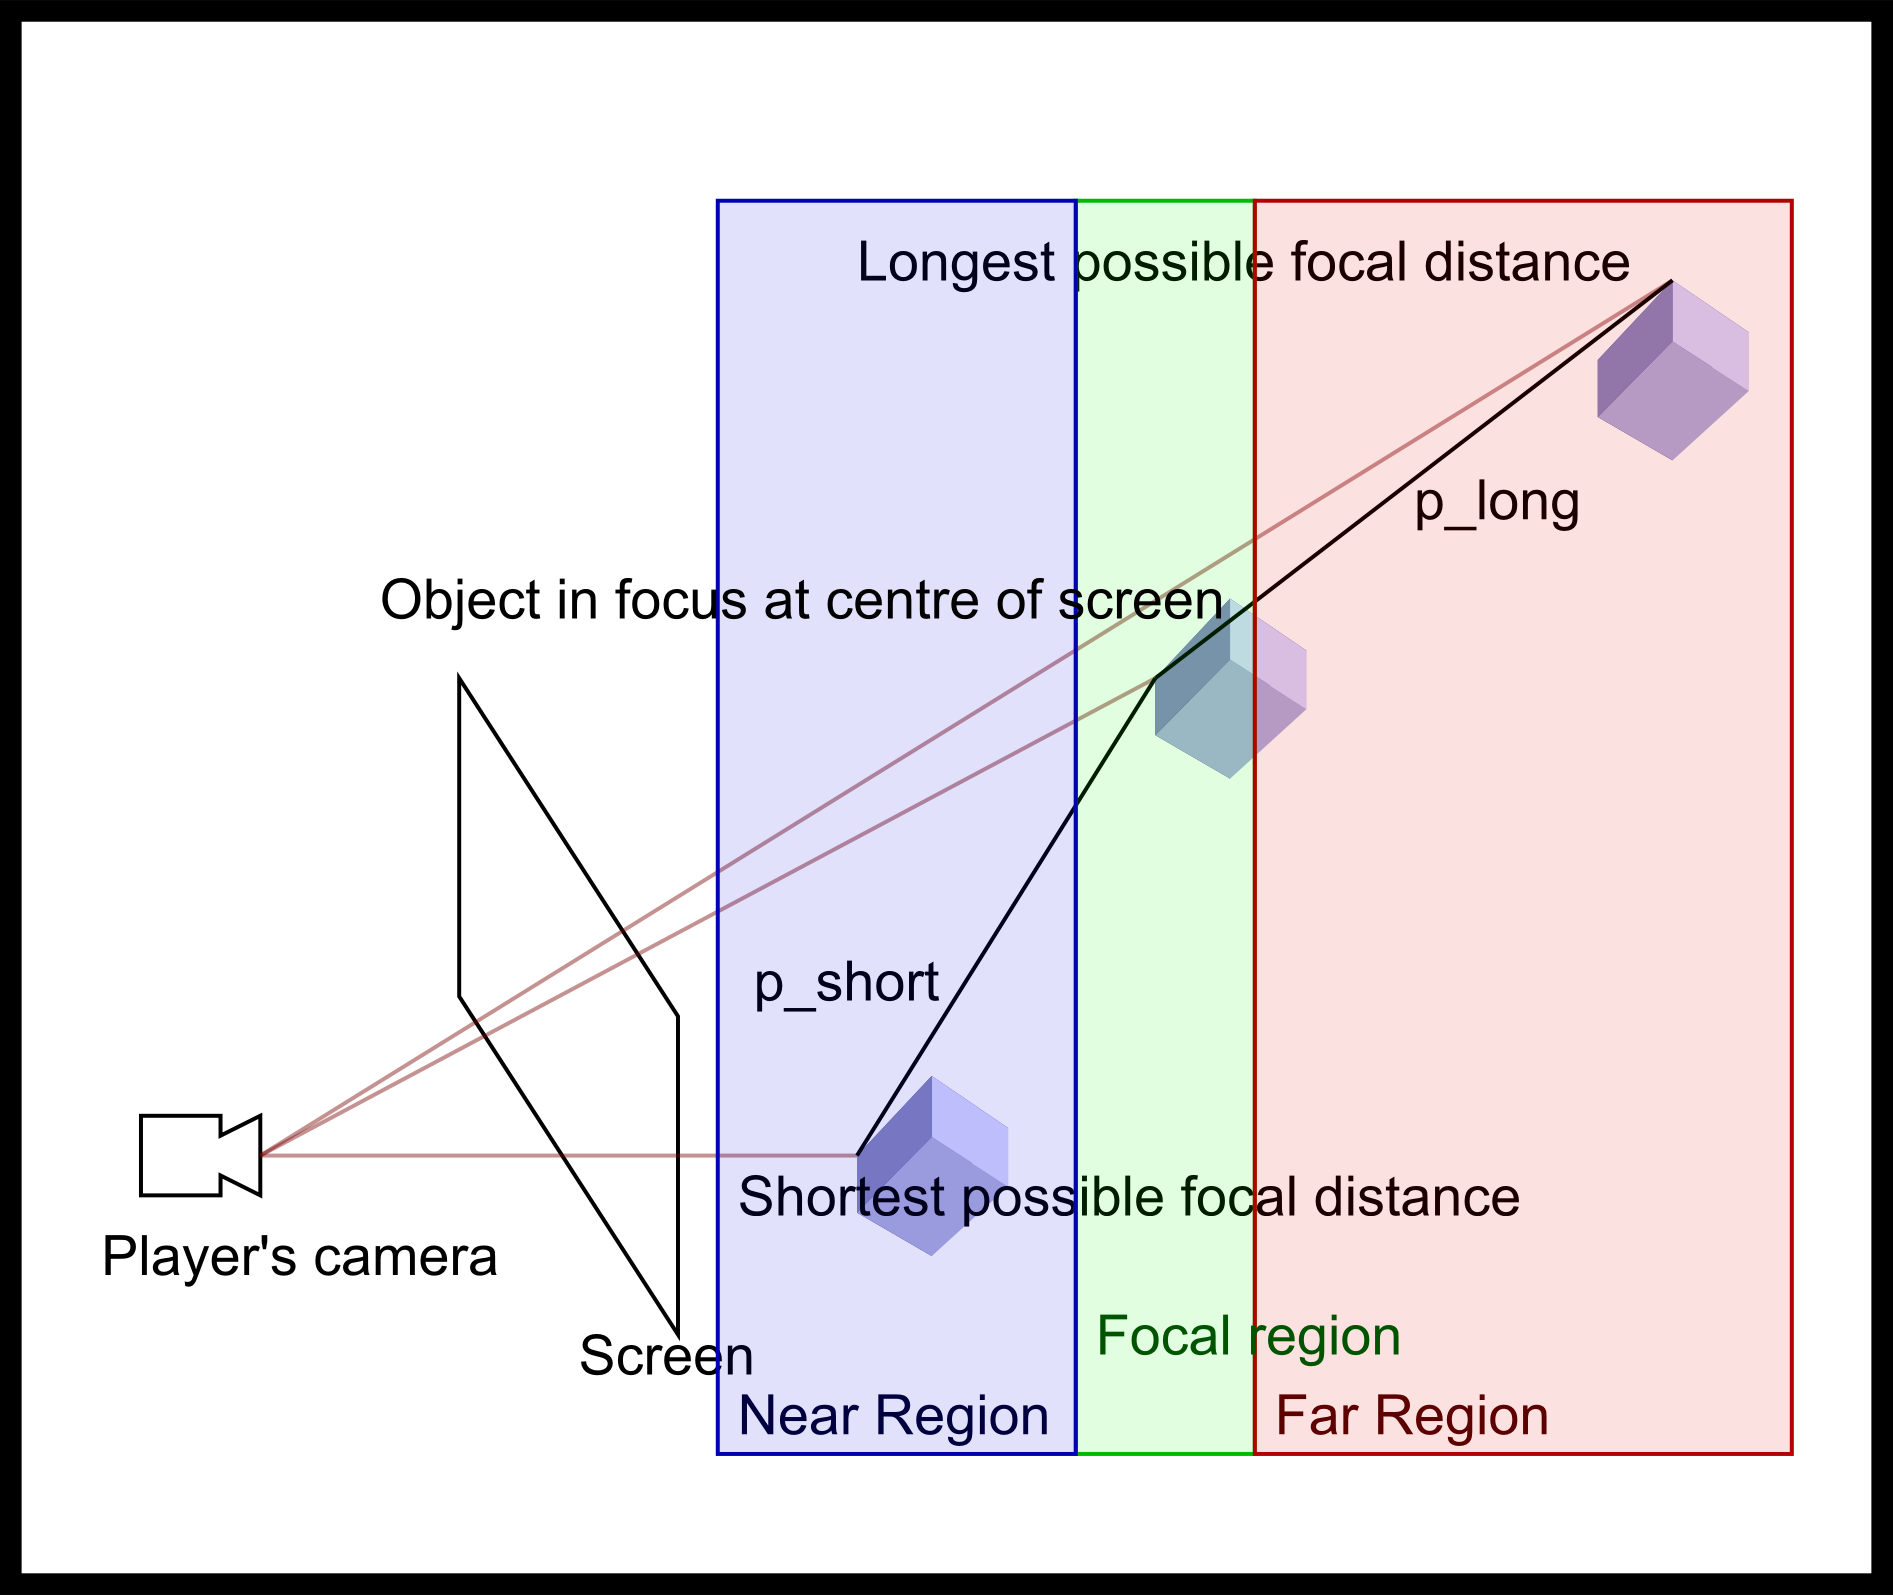
\includegraphics[width=0.45\textwidth]{images/bokehDOF.png}
%           \caption{The setup for bokeh DoF. {\color{blue} [TODO: caption]}}
%            \label{fig:raycast}
%\end{figure}
%
%We then split the screen into three regions: the near, far and focal regions. The focal region is the set of pixels whose object distances are within $100cm$ of $d_{centre}$. The far region consists of all pixels with object distances further than this, and the near; all pixels with smaller object distances.\\

%For each pixel in the near region, we define $p_c$ as the world space distance between the object under the pixel and the object under the pixel at the centre of the screen. We then construct a Circle of Confusion for each pixel, using a textured quad containing a circular bokeh opacity texture. This circular texture has a radius $r = D_c * \frac{p_c}{p_{short}}$ and an opacity proportional to this radius. \\
%
%To move the focal regions we cast a ray from the center of the participants stereo 3D view on the Oculus into the scene, and find the distance $D$ at which this ray first intersects an object. We then create a circle of radius $r_c = \frac{D}{C_c}$ ($C_c$ is constant) and randomly cast $n$ rays into this circle, with a weighting towards rays clustered in the center, each of which reports a distance $d_{0..n}$. We then iteratively cull outlier distances from this set and take the mean distance until a confident final focal distance $d_f$ is found. $d_f$ is then compared to the prior focal distance and interpolated based on .\\
%
%\begin{figure}[h!]
 %       \centering
 %           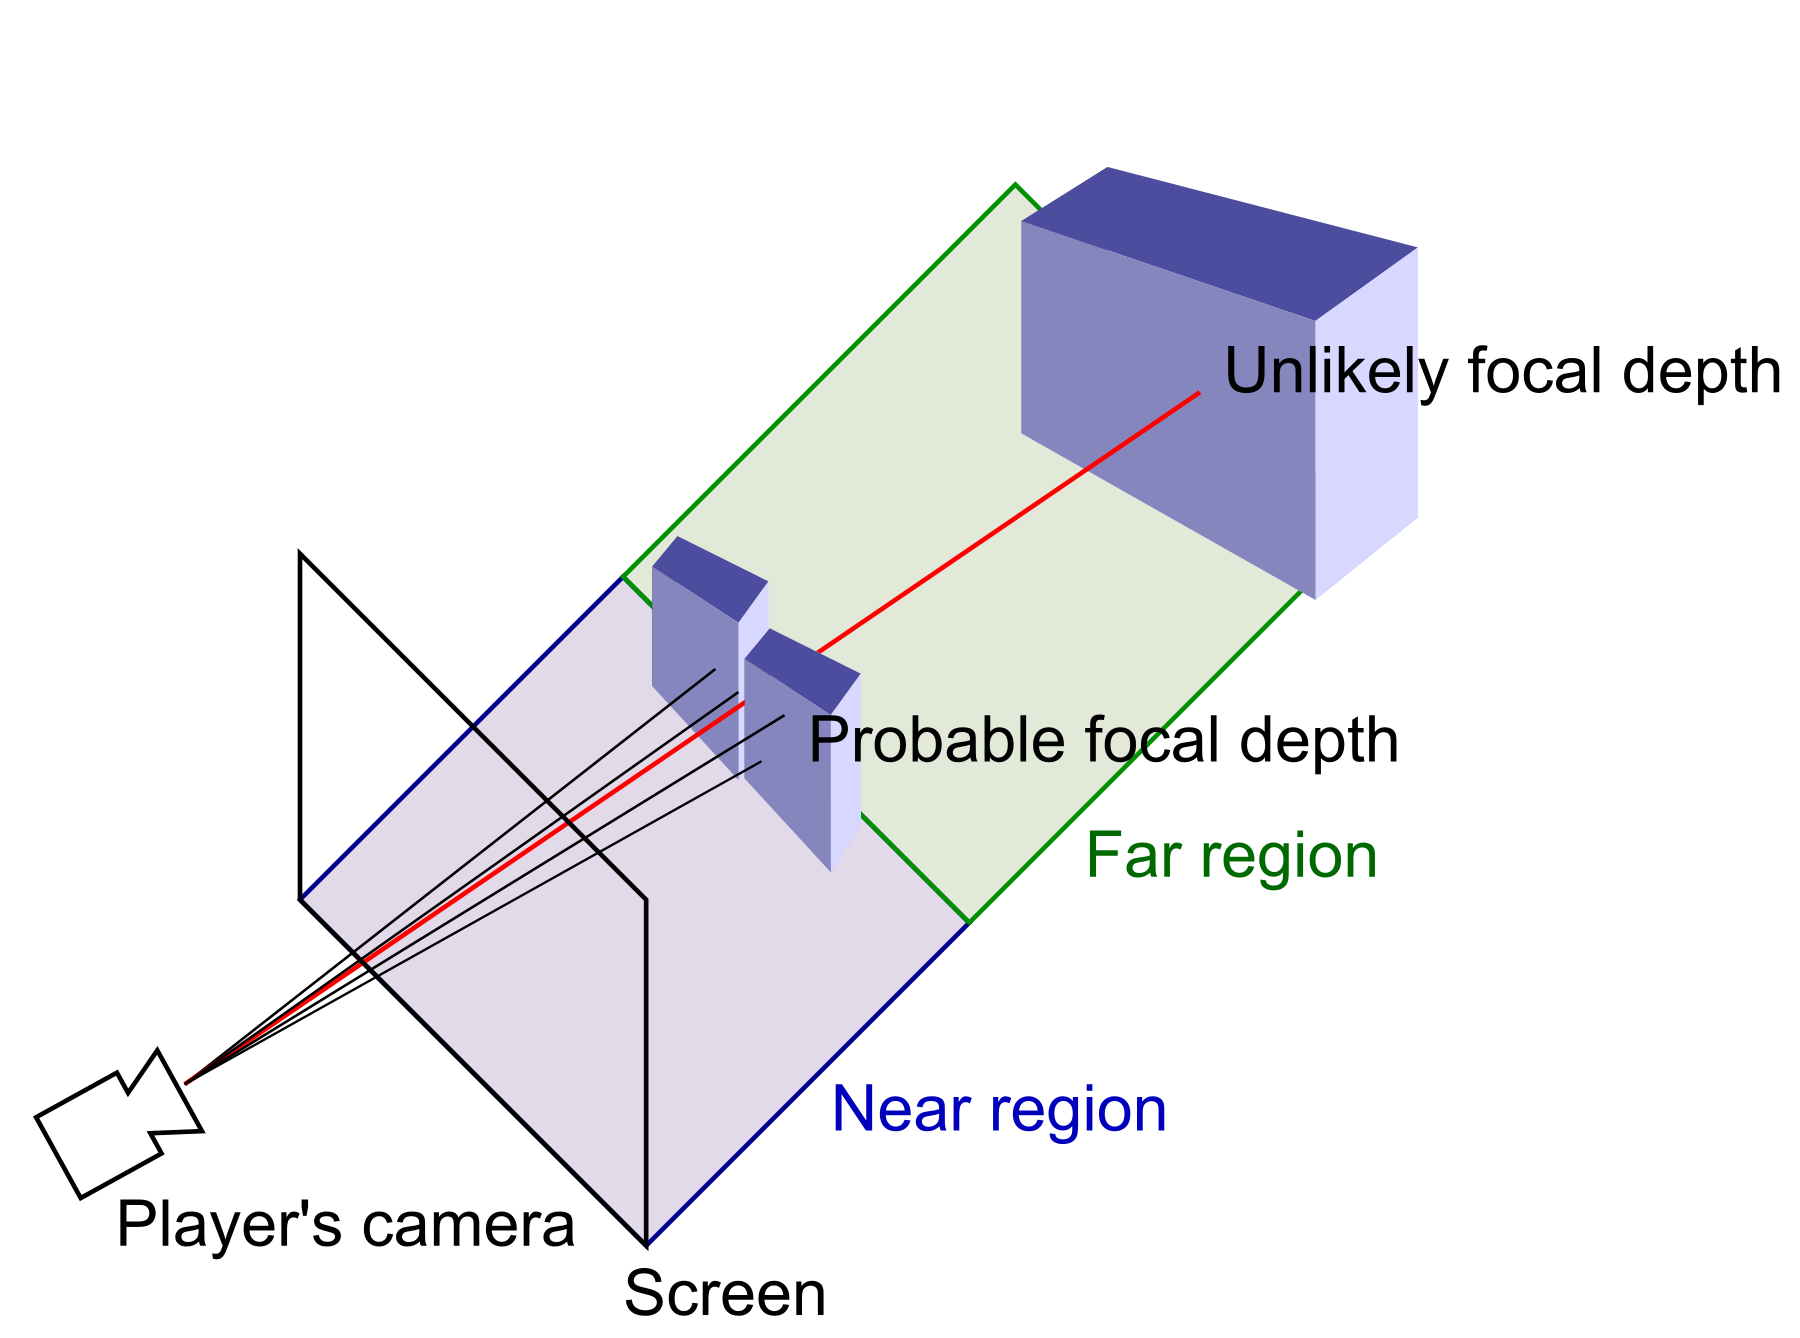
\includegraphics[width=0.45\textwidth]{images/distanceCheck.png}
%            \caption{In order to ensure focus on the correct object, rays (grey) are cast into the circle around the object under the centre of the screen (black ray).}
%            \label{fig:bokeh}
%\end{figure}
%REWORDING END


Participants completed the study on a machine running Windows 7 with 8GB RAM, a 3.6GHz Intel quadcore CPU and a NVIDIA GTX 770 GPU with an attached Oculus Rift DK1 HMD. An example picture of the experimental set-up is shown in Fig.~\ref{fig:user}. 
\\

\begin{figure}[h!]
        \centering
            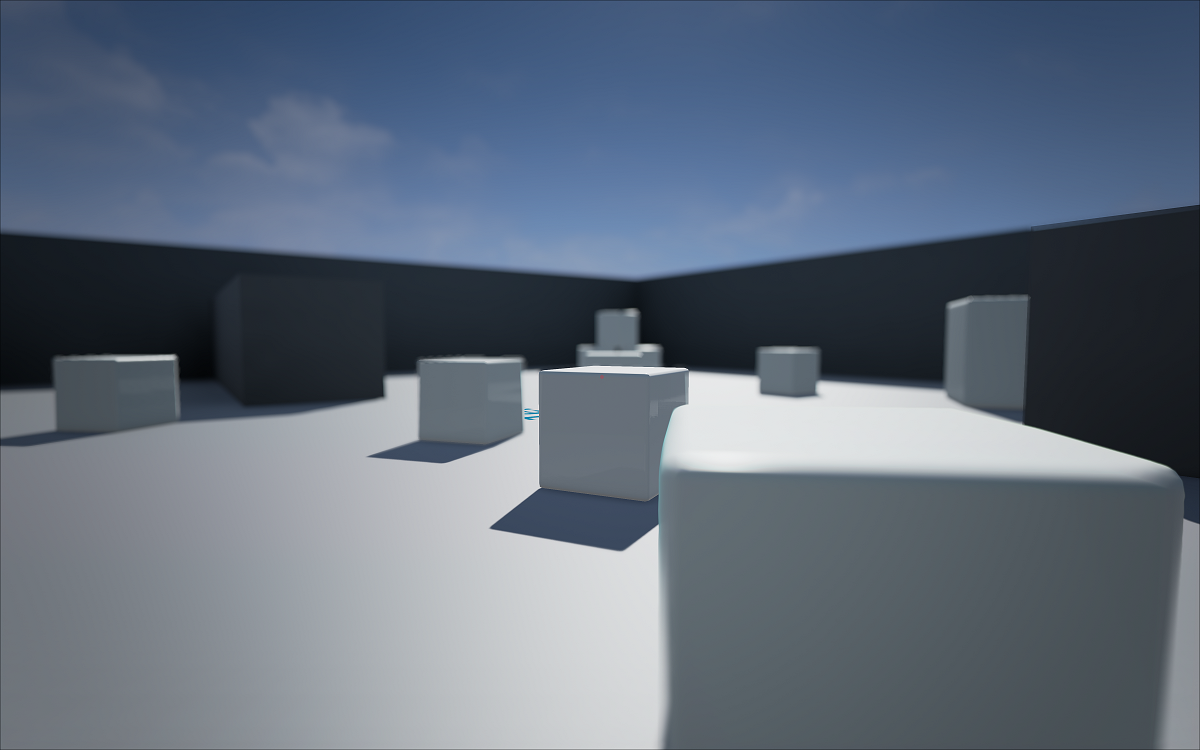
\includegraphics[width=0.45\textwidth]{images/testScene.png}
            \caption{The test scene used for selecting DoF blur radius}
            \label{fig:testScene}
\end{figure}

% thrhee comment: the following needs to be removed
% We utilize the bokeh DOF provided in provided in UE4 as the UE4 implementation is both high quality and fast. The above process is completed at quarter resolution (half vertical and horizontal). No artefacts or errors are visible from this, due to the low resolution of the Oculus screen.\\

% no fine detail
% focal gradient / etc


% The followings are not required
% We chose the Oculus DK1 over more recent devices, such as the Oculus DK2 due to the lower hardware requirements to optimally run the DK1. Furthermore, the DK2, being newer, does not have the same level of software support that the DK1 offers, and was at the time of our study, known to have performance issues.{\color{blue}[Do I need to cite this?]}. An example picture of the experimental set-up is shown in Figure \ref{fig:user}\\

\begin{figure}[h]
        \centering
            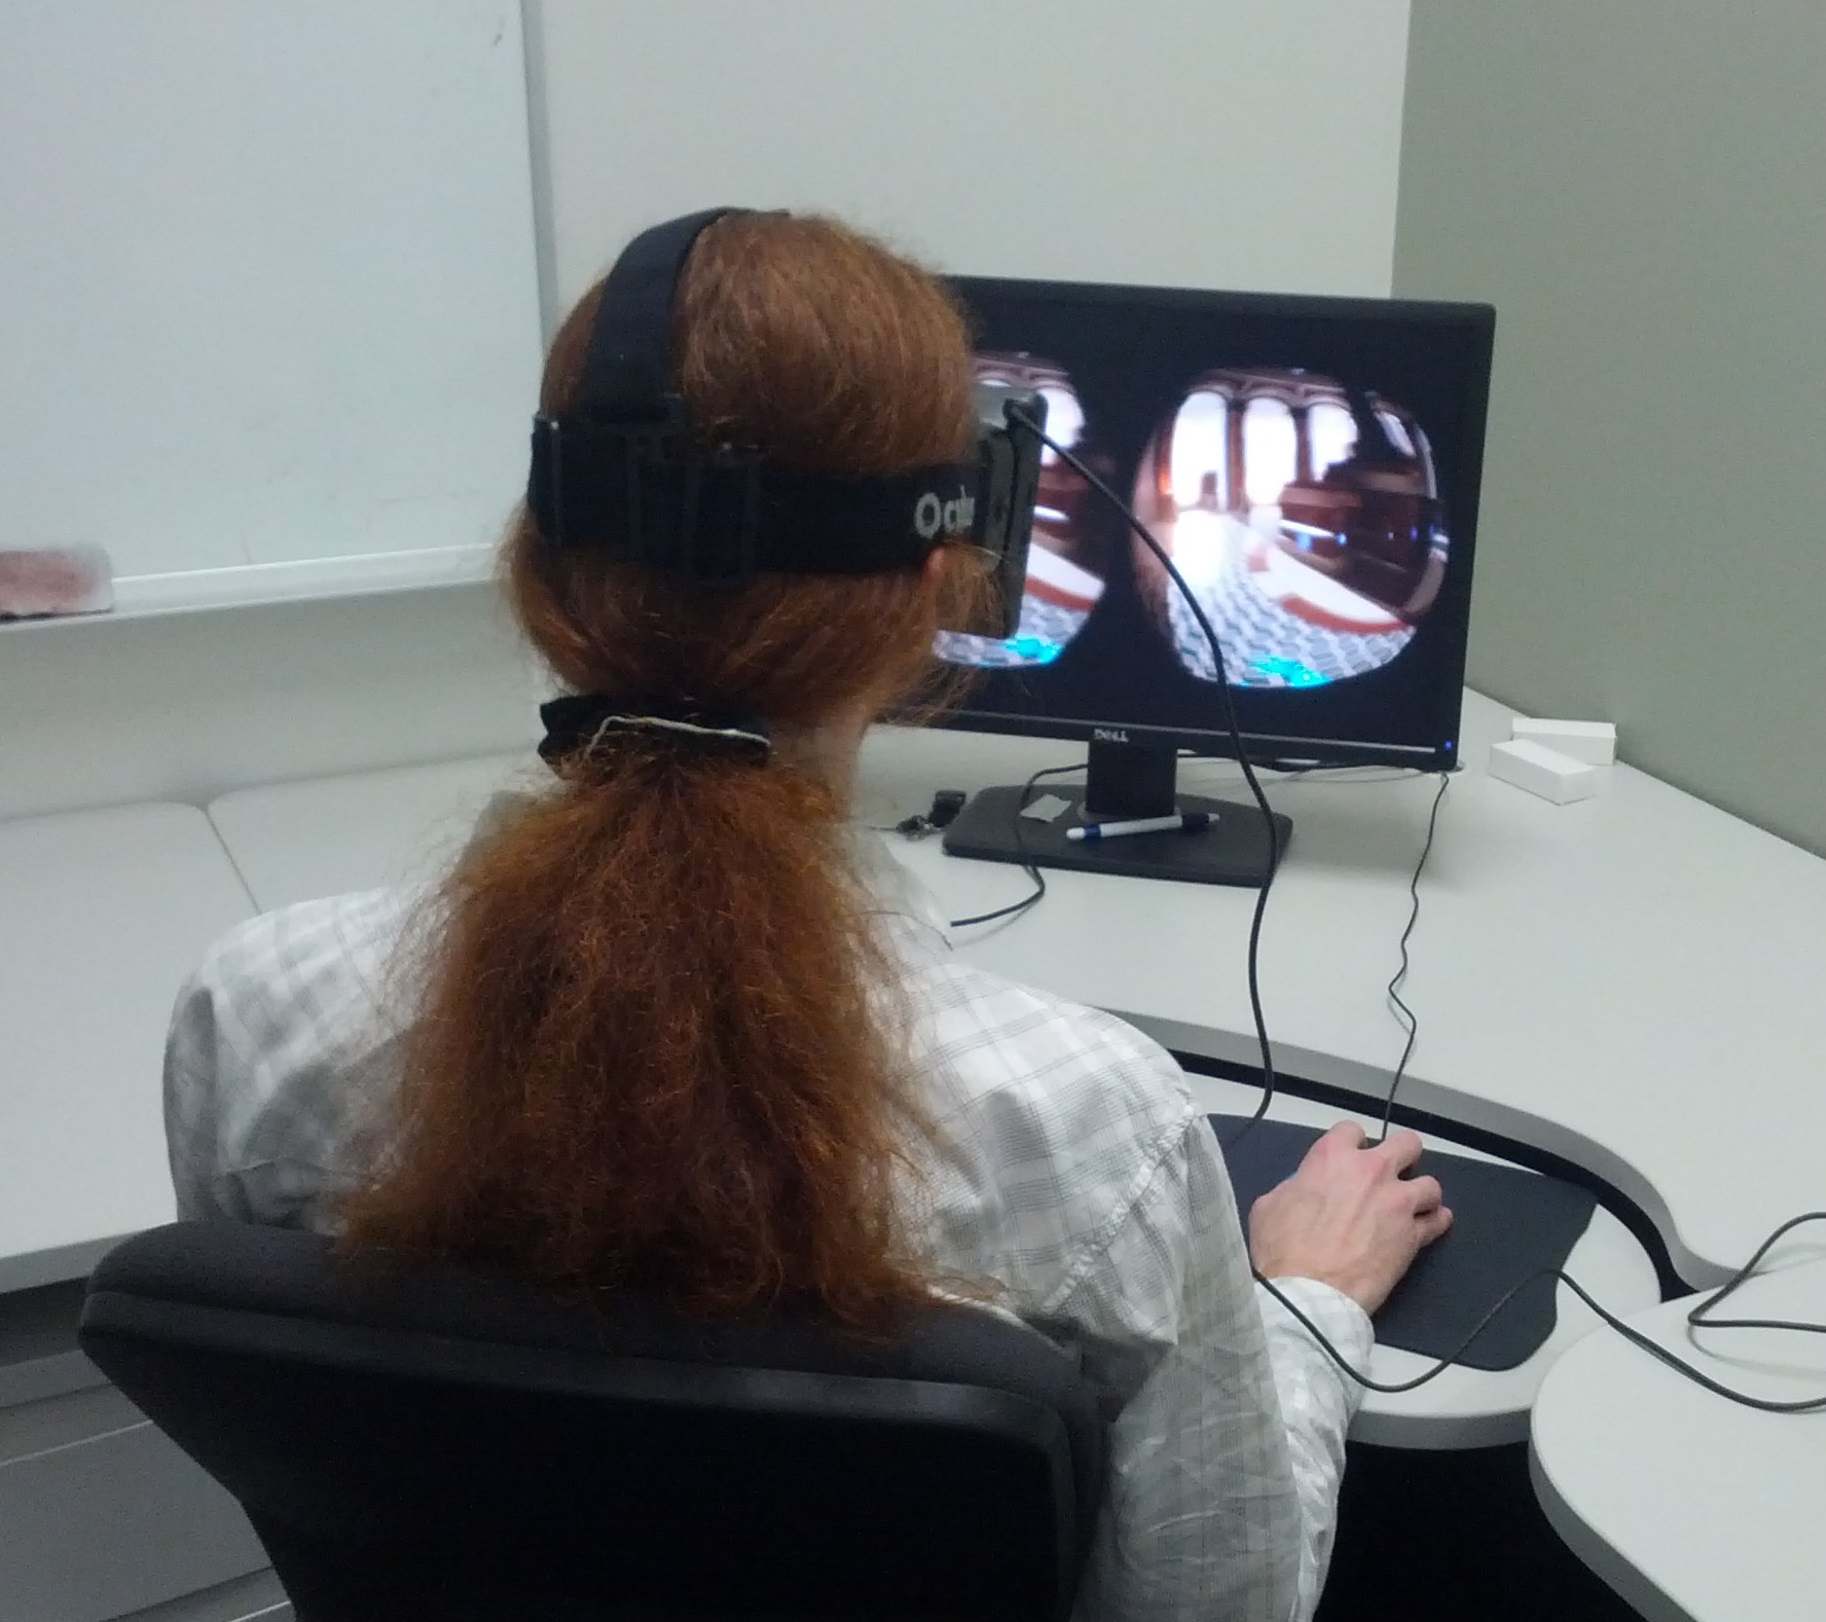
\includegraphics[width=0.45\textwidth]{images/participantv2.jpg}
            \caption{A participant during the user study.}
            \label{fig:user}
\end{figure}

